\documentclass{article}
\usepackage[utf8]{inputenc}
\usepackage{amsmath,amsthm,amssymb,amsfonts,mathtools}
\usepackage[a4paper, total={6.5in, 10.2in}]{geometry}
\usepackage{graphicx}
\usepackage{charter}
\usepackage{tabto}
\usepackage[colorlinks = true,
            linkcolor = blue,
            urlcolor  = blue,
            citecolor = blue,
            anchorcolor = blue]{hyperref}
\usepackage{newtxmath}
\usepackage{thmtools}
\usepackage{float}
\usepackage{enumerate}
\usepackage{tikz}
\usepackage{cleveref}
\usepackage[most]{tcolorbox}

\newtcbtheorem[auto counter, number within=section]{theorem}{Theorem}
{colback=red!5,colframe=red!35!black,fonttitle=\bfseries,breakable}{th} 
% \newtheorem{theorem}{Theorem}[section]%
\newtheorem{definition}{Definition}[section]
\newtheorem{corollary}{Corollary}[section]
\newtheorem{example}{Example}[section]
\newcommand{\R}{\mathbb{R}}
\newcommand{\Rw}{\Rightarrow}
\newcommand{\hs}{\hspace}
\newcommand{\vs}{\vspace}
\newcommand{\ds}{\displaystyle}
\renewcommand{\qedsymbol}{$\blacksquare$}
\usepackage{titlesec}

\title{\textbf{\huge{Real analysis}}}
\author{Abrar Akib \\[3ex]
\begin{minipage}[t]{15cm}\small\centering\text{Link to the code can be found\;\href{https://github.com/abrar2akib/codes_of_latex/real-analysis/main.tex}{here}} \end{minipage}}
\titleformat{\section}
  {\normalfont\Large\bfseries}{\thesection}{1em}{}[{\titlerule[0.8pt]}]

\begin{document}

\maketitle
\tableofcontents
\listoftheorems
\section{Introduction}
\textbf{Statement:} That has to be proved. It can be either true or false. There will be no vague answer.\\
\textbf{Tautology:} Statement which are always true. $x^2<x$ when$ 0<x<1$
    \begin{table}[H]
        \centering
        \scalebox{1.3}{
            \begin{tabular}{|c|c|}
            \hline Operators & Symbol \\ \hline\hline
            And & $\wedge$ \\ \hline
            Or & $\vee$ \\ \hline
            If...then & $\Rw$ \\ \hline
            If and only if & $\Leftrightarrow$\\ \hline
            Negation/ not & $\neg$ \\ \hline
            Equivalent & $\equiv$\\ \hline
            \end{tabular}}
        \caption{ Symbol of the operators}
        \label{tab:mylabel}
    \end{table}
\textbf{Contra positive: } If the statement is $P\ \Rw \ Q$ then its contra positive will be $\neg \ Q \Rw \neg \ P$. \\\\
Example : If P= "Present in Dhaka" and Q="Present in Bangladesh" \\ Then P implies Q but Q does not implies P.\\ Now $\neg \ P$ = "Not in Dhaka" and $\neg \ Q$ ="Not in Bangladesh" \\ then only $\neg \ Q \Rw \neg \ P$ is true and the opposite is not.\\
\textbf{Converse: } If the statement $P\ \Rw \ Q$ is true then $Q\ \Rw \ P$ may not always be true.
\subsection{Methods of Proofs:}
\begin{enumerate}
    \item \textbf{Direct Method:} If $P\ \Rw \ Q$, here P implies Q assuming P is true. Our target is to prove Q is true. We start from P then we get to a logical step in a row then we reach a conclusion.\\
    $P \Rw R_1 \Rw R_1 \Rw R_1 ... \Rw Q$\\\\
    \begin{example}
        The square of an odd integer is also odd.
        \begin{proof}
            Let, n be an odd integer. i.e. $n=2K-1 \qquad \forall K \in \mathbb{R} $ \\
            so,
            \begin{align*}
                n^2 &= (2K-1)^2 \hs{12cm}\\
                &= 4K^2-4K+1\\
                &= 4K^2-4K+2-1\\
                &= 2(2K^2-2K+1)-1\\
            \end{align*}
            By properties of integer, $2K^2-2K+1=m$ is also an integer. So $2m^2-1=n^2$ is also an odd integer.
        \end{proof}
    \end{example} 
    \item \textbf{Proof by Contradiction: } If we want to prove $P \Rw Q$ \\
        We first assume Q is not true. i.e. $P \Rw \neg Q$. From here we will go through some logical steps and eventually will face a contradiction that violates our initial assumption.
    \begin{theorem}{\empty}{\empty}
        Prove that, $\forall a \in \mathbb{R^{++}},\quad a^-1>0$
        \begin{proof}{By contradiction}
        Let's assume, $\forall a> 0, \qquad a^-1<0$\\
           By order properties, $a.a^-1 \Rw 1<0$ \\
           It is a contradiction $\therefore \forall a >0, \quad a^-1>0$\\
                \end{proof}
    \end{theorem}
    \item \textbf{Mathematical Induction: } There are some statements related to natural numbers. We use this method for those proofs. i.e.\\
    $\displaystyle 1+2+3+....+n = \frac{n(n+1)}{2}$\\
    Here we will prove it for n=1. Then if it is true for n=1 then it will be true for any other values of n.\\
    \textbf{Initial step:} P is a statement and it is true for 1. P(1) is true.\\
    \textbf{Induction step:} We will assume P(n) \textit{[Induction hypothesis]} is true, and will try to prove that P(n+1) is also true.        
    \begin{example}
        $\displaystyle 1+2+3+....+n = \frac{n(n+1)}{2}$\\
        \begin{proof}
            \textbf{Initial step:} For n=1 , $\displaystyle \frac{1(1+1)}{2}=1$ \textit{[this is trivial]}\\
            \textbf{Induction step: } Assume, $\displaystyle 1+2+3+....+n = \frac{n(n+1)}{2}$ is true. Now we have to prove this is true for (n+1).
            \begin{align*}
                1+2+3+...+n+(n+1)\\
                \Rw & \frac{n(n+1)}{2}+(n+1) \hs{5cm} \text{[By induction hypothesis]}\\
                \Rw & \frac{n(n+1)+2(n+1)}{2}\\
                \Rw & \frac{(n+1)(n+2)}{2}\\
                \Rw & \frac{(n+1)\{(n+1)+1\}}{2}\\
            \end{align*}
            $\therefore$ The statement is true.
        \end{proof}
    \end{example}
\end{enumerate}
\subsection{Field {$\mathbb{F}$}}
\begin{definition}
    Field is a set of elements with two operations: addition (+) and multiplication (*). Consists of same type of elements (matrices, functions)\\\\
\end{definition}
\textbf{Additive properties/axioms:} $\forall a,b,c \in \mathbb{F}$
\begin{enumerate}
    \item $ a+b=b+a $
    \item $ (a+b)+c=a+(b+c)$
    \item   $\exists\; 0 \text{such that}\quad 0+a=a$
    \item   $\exists \;-a, \text{such that}\quad a+(-a)=0$
\end{enumerate}
\textit{[Here 0 and -a should not necessarily exist in the field ]}\\\\
\textbf{Additive properties/axioms:} $\forall a,b,c \in \mathbb{F}$
\begin{enumerate}
    \item $a.b=b.a $
    \item $(a.b).c=a.(b.c)  $
    \item $\exists \;1 ,\;\text{such that}\quad 1.a=a $
    \item $\exists \;a^{-1}, \text{such that}\quad a.a^{-1}$ 
    \item Distributive: $a.(b+c)=a.b+a.c$
\end{enumerate}
$\mathbb{N}$ is not field as it does not include  0 in it. 
Also, $\mathbb{Z}$ is not field as it does not include  fractions in it.
But, $\mathbb{Q,R,C}$ are field. \\\\
Set of (2x2) matrices is not field. As these do not follow multiplicative commutative property.
\begin{theorem}{}{}
    We can write $\forall a \in \R,\;0.a=0$
\begin{proof}We know,
    \begin{align*}
              & 0+0 = 0                         & \text{[Additive identity]}             \\
        \Rw\; & (0+0).a  = 0.a                  & \text{[Multiplying both sides with a]} \\
        \Rw\; & 0.a + 0.a=0.a                   & \text{[Distributive]}                  \\
        \Rw\; & (0.a)+(0.a)+(-0.a)=(0.a)+(-0.a) & \text{[Additive Inverse]}              \\
        \Rw\; & 0.a+0=0 \hs{5cm}                & \text{[Additive Identity]}             \\
        \Rw\; & 0.a=0                                                                    \\
    \end{align*}
\end{proof}
\end{theorem}
\begin{theorem}{}{}
    If $a,b \neq 0$, then $(ab)^{-1} = a^{-1}.b^{-1}$
\begin{proof}
    \begin{align*}
        (a^{-1}.b^{-1})(ab)
         & = (a^{-1}.b^{-1})(ba) \hs{4cm} & \text{[Commutative]}             \\
         & = a^{-1}(b^{-1}b)a             & \text{[Associative]}             \\
         & =a^{-1}.1.a                    & \text{[Multiplicative Inverse]}  \\
         & =a^{-1}.a                      & \text{[Multiplicative Identity]} \\
         & =1                             & \text{[Multiplicative Inverse]}
    \end{align*}
    Now,
    \begin{align*}
              & (a^{-1}.b^{-1})(ab)=1  \hs{6cm}                                   \\
        \Rw\; & a^{-1}b^{-1}ab(ab)^{-1}=1                                         \\
        \Rw\; & a^{-1}b^{-1}=1(ab)^{-1}         & \text{[Multiplicative Inverse]} \\
        \Rw\; & a^{-1}b^{-1}=(ab)^{-1}                                            \\
    \end{align*}
\end{proof}
\end{theorem}
\subsection{Order Properties}
\begin{enumerate}
    \item \textbf{Trichotomy property: } \\
If $a,b \in \mathbb{F}$ then exactly one of three things is possible: $a<b$ or $b<a$ or $a=b$\\
\textbf{Another version:} if $a\in \mathbb{F}$, then exactly one of the three things is possible. $a<0,\; a>0,\; a=0$
    \item \textbf{Transitivity property: }\\
$\forall a,b,c \in \mathbb{F} $ if $a<b$ and $b<c$ then $a<c$
\item $\forall a,b,c \in \mathbb{F}$
        \begin{itemize}
            \item if $a<b$ then $a+b<b+c,\;\forall c \in \mathbb{F}$ 
            \item if $a<b$ and $c>0$ then $ac<bc$\\\\
        \end{itemize}
\end{enumerate}
\textbf{Question: } Complex numbers do not follow he order properties.
\begin{proof}
    x=a+bi is a complex number where $i=\sqrt{-1}$ and $a,b \in \mathbb{R}$\\
    \begin{align*}
        \text{Let,} &i>0\\
        \Rw \;& i.i>0.i \hs{5cm}\text{[By order property]}\\
        \Rw \;& i^2>0\\
        \Rw & -1>0\\
    \end{align*}
    Which is a contradiction. Similarly, assuming $i\leq0$ will lead to a contradiction.\\
    $\therefore$ Complex numbers do not follow the order properties.
\end{proof}
\begin{example}
    Prove that, $1>0$
    \begin{proof}(Proof by contradiction)\\
        \textbf{Case 1:} Assume, 1=0\\
        let $a\in\mathbb{R}$ such that $a\neq 0$\\
        Now, $a=a.1=a.0=0$\\
        Which is a contradiction\\\\
        \textbf{Case 2: } Assume $1<0$\\
        let $a\in\mathbb{R}$ such that $a\geq 0$\\
        Now, $1<0 \Rw 1.a < 0.a \Rw a < 0$\\
        Which is a contradiction\\\\
        Therefore, by Trichotomy property $1>0$\\
    \end{proof}
\end{example}
\textit{[According to our third order property we have seen that our sign relationship remains unchanged when multiplied with a positive number. What happens when we multiply with a negative number?]}
\begin{theorem}{}{}
     If $a<b$ and $c<0$, then $ac>bc$.\\ 
    \begin{proof}
         Here, $c<0 \Rw -c>0$(why?)\\
    \begin{align*}
        \text{Now,}\quad &a<b \hs{7cm}\\
        \Rw\;& a(-c)<b(-c) &\text{[Order property]}\\
        \Rw\;& -ac<-bc\\
        \Rw\;& -ac+ac+bc<-bc+ac+bc  &\text{[Order property]}\\
        \Rw\;& 0+bc<-bc+bc+ac       &\text{[Commutative property]}\\
        \Rw\;& bc<0+ac             &\text{[Additive Inverse and identity]}\\
        \Rw\;& bc<ac                &\text{[Additive Identity]}
    \end{align*}
    \end{proof}
\end{theorem}
\subsection{Completeness Property}
\begin{definition}
    Completeness is a property of the real numbers that, intuitively, implies that there are no "gaps" or "missing points" in the real number line. This contrasts with the rational numbers, whose corresponding number line has a "gap" at each irrational value.
\end{definition}   
    Suppose, $S\subseteq R$ and S is non-empty. 
    \begin{itemize}
        \item If $\forall u \in \mathbb{R}$ and $u\leq s,\; \forall s \in S$ then we say S is bounded below and each such u is called lower bound of S.\\
        \item If S is bounded below, then v is infimum(greatest lower bound) of S when:
            \begin{enumerate}[i.]
                \item v is a lower bound
                \item $v \geq u, \forall u$ in lower bound
            \end{enumerate}
        \item If $\forall w \in \mathbb{R}$ and $w\geq s,\; \forall s \in S$ then we say S is bounded above and each such w is called upper bound of S.\\
        \item If S is bounded above, then t is supremum(Least upper bound) of S when:
            \begin{enumerate}[i.]
                \item t is an upper bound
                \item $t \leq w, \forall w$ in upper bound
            \end{enumerate}
    \end{itemize}
\begin{figure}[H]
    \centering
    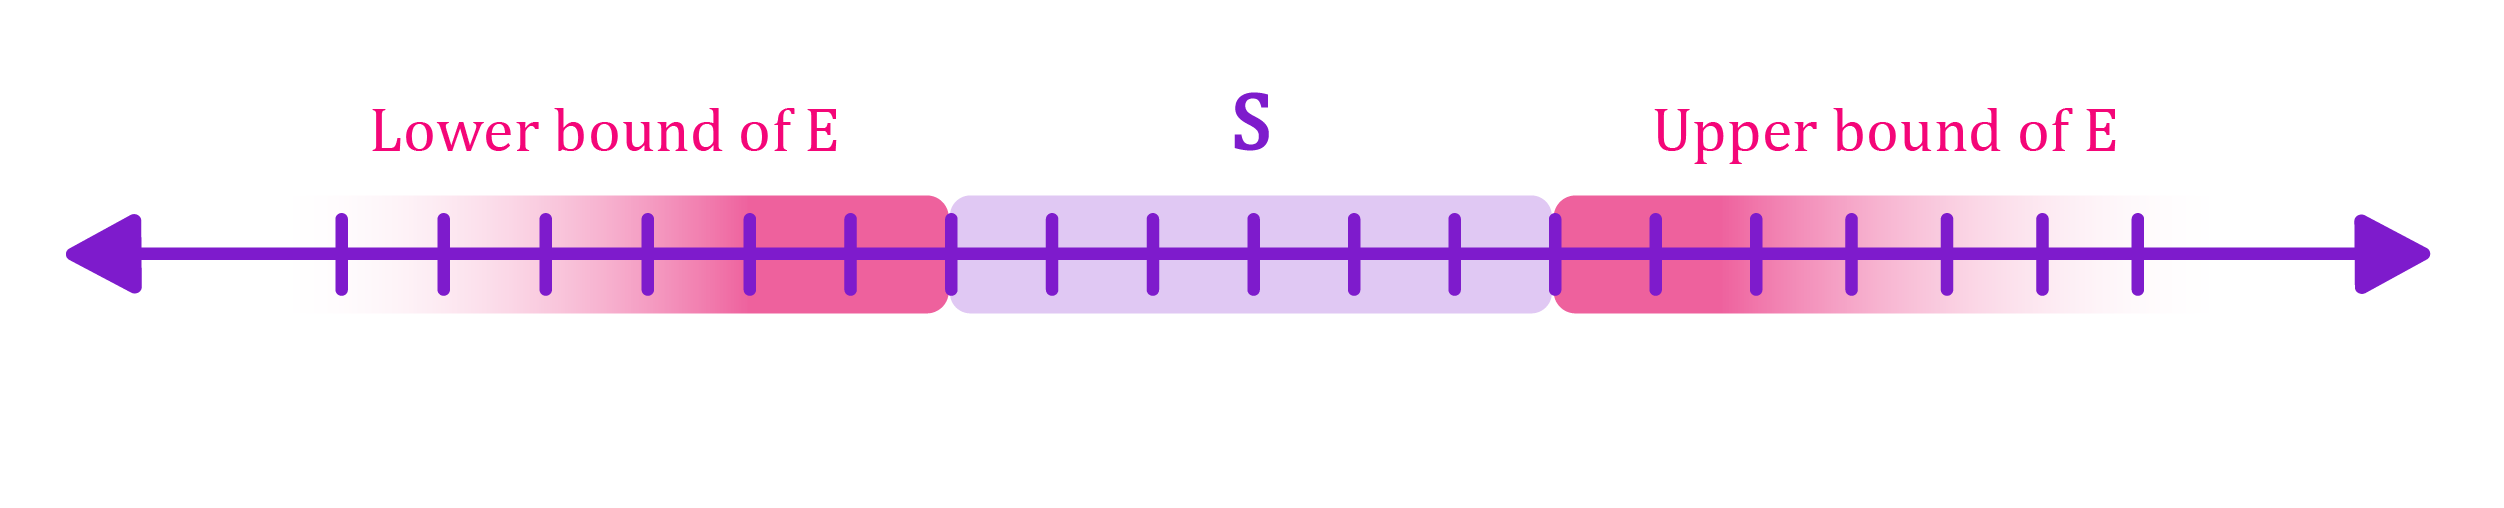
\includegraphics [width=10cm,height=10cm,keepaspectratio]{tex graphs-11.png}
    \caption{Least upper bound}
\end{figure}
\begin{flushleft}\large{Completeness property $\equiv $ Least upper bound property}\end{flushleft}
An ordered set S is said to fulfill the completeness property, if for all non empty subset $E\subset S$ which are bounded above, there exists a least upper bound of E in S.\\
\begin{figure}[H]
    \centering
    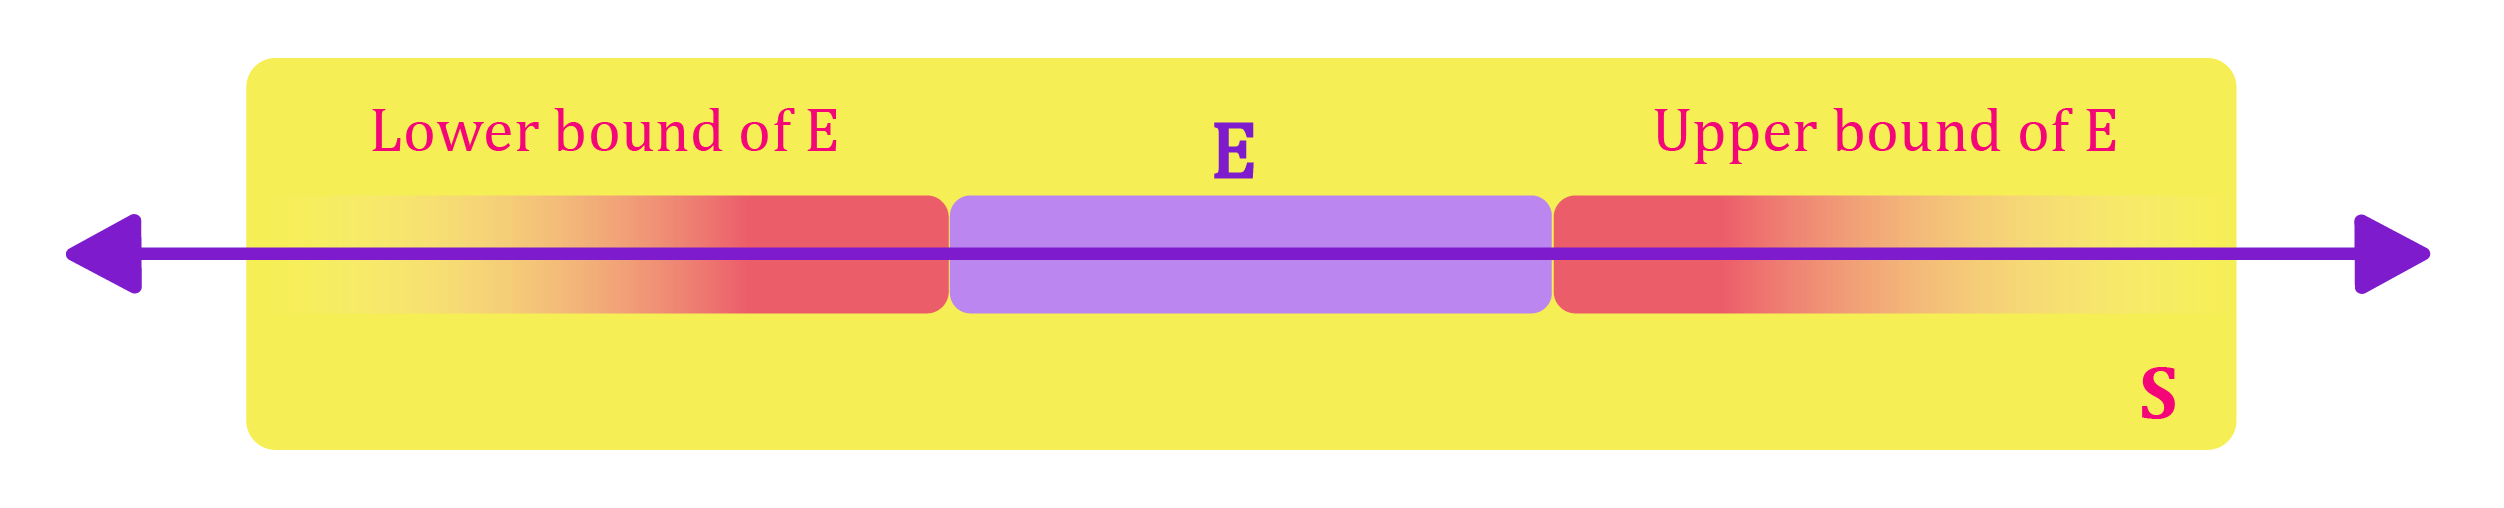
\includegraphics [width=10cm,height=10cm,keepaspectratio]{tex graphs-12.png}
    \caption{Lower and upper bound}
\end{figure}
\begin{example}
    $\mathbb{Q}$ is the set of rational number.\\
    Subset, $E=\{x\in\mathbb{Q}\;|\;x^2<2\}$\\
    Here, E is bounded above because $\exists M$ such that $M^2\geq2$\\
    Here least upper bound is $\sqrt{2}$ But $\sqrt{2} \notin \mathbb{Q}$
    \begin{figure}[H]
    \centering
    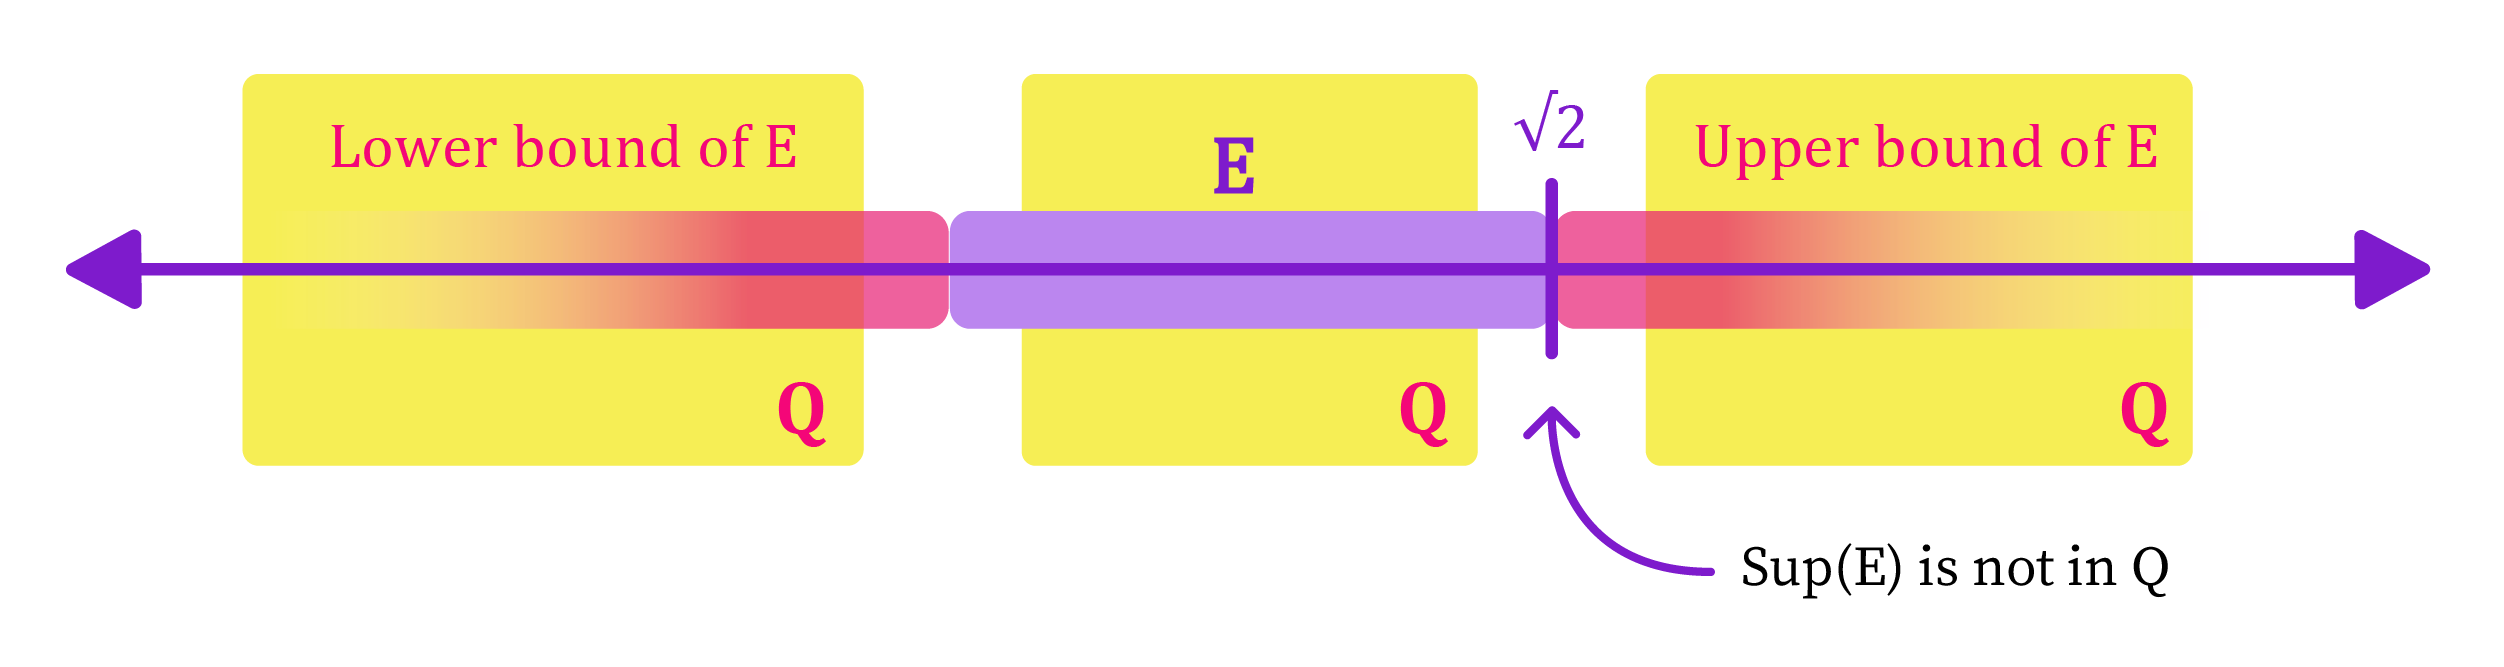
\includegraphics [width=10cm,height=10cm,keepaspectratio]{tex graphs-13.png}
    \caption{Least upper bound}
\end{figure}
\end{example}
\textit{[Real number line is a complete ordered field.(why?)]}
\subsection{Archimedean Property}
An ordered field (i.e. $\mathbb{R}$) is archimedean if $\forall x \in \mathbb{R}, \exists n \in \mathbb{N}$ such that $x<n$. Whatever x we take we will always be able to find a greater n as $\mathbb{N}$ is not bounded above.
\begin{proof}
    \textit{(By contradiction)} \\
    Let's assume, $n\leq x$ [ which entails that $\mathbb{N}$ is bounded above]\\
    So, x is upper bound of $\mathbb{N}$. We know that $\mathbb{N} \subset \mathbb{R}$\\\\
    By completeness property, $\mathbb{N}$ has a supremum in $\mathbb{R}$. Say u be that supremum. So, $u \in \mathbb{R}$\\
    Now $u-1<u$ So, (u-1) is not the least upper bound. \\
    This implies $\exists m \in \mathbb{N}$ subject to $u-1<m \Rw u<m+1$\\
    But $m-1 \in \mathbb{N}$ which means a value in $\mathbb{N}$ is greater that its own supremum. This contradicts that u is the supremum. \\\\
    Therefore, $x<n$
\\\\
\textbf{Another version: } If $r,s \in \mathbb{R}^{>0} $ then $\exists n \in \mathbb{N}$ such that $r<ns$. \\
since, $s>0,\ s^{-1}>0$\\
By order property, $rs^-1>0$  [r and s are positive]\\
Now, by archimedean property,\\
$\exists n \in \mathbb{N}$ subject to $rs^-1<n$\\
so, $rs^-1.s<ns$\\
$\Rw r < ns$
\\\\
\textbf{Density Property:}\\
Rational number $\mathbb{Q}$ are dense in real number $\mathbb{R}$. In another words, between two real numbers we will get a real number. 
\end{proof}
\begin{theorem}{(1)}{}
    If z and a are elements in $\mathbb{R}$ with $z+a=a$ then $z=0$
    \begin{proof}
        \begin{align*}
            & z+a=a\\
            \Rw \ & z+a+(-a)=a+(-a)\hs{3cm}\textit{[adding (-a) to both sides]}\\
            \Rw \ & z=0 \hs{3cm}\textit{[additive inverse]}\\
        \end{align*}
    \end{proof}
\end{theorem}
\begin{theorem}{(2)}{}
    If $u \neq 0$ and $b \neq 0$ are elements in $\mathbb{R}$ with $u.b=b$ then $u=1$
    \begin{proof}
        Here, 
        \begin{align*}
            &u.b=b\\
            \Rw \ & u.b.(b^-1)=b.(b^-1)\hs{3cm}\textit{[Multiplying both sides by $b^{-1}$]}\\
            \Rw \ & u=1 \hs{3cm}\textit{[Multiplicative inverse]}\\
        \end{align*}
    \end{proof}
\end{theorem}
\begin{theorem}{(3)}{}
    Ia $a\in \mathbb{R}$ then $a.0=0$
    \begin{proof}
        \begin{align*}
            a.0 & =a.0+0 (Additive identity)\\
                & =a.0+(a+(-a)) \hs{3cm}\textit{[Additive inverse]}\\
                &=(a.0+a)+(-a) \hs{3cm}\textit{[Associativity]}\\
                &=(a.0+a.1)+(-a) \hs{3cm}\textit{[Multiplicative identity]}\\
                &=a.(0+1)+(-a)\hs{3cm}\textit{[Distributivity]}\\
                &=a.1+(-a) \hs{3cm}\textit{[Additive identity]}\\
                &=a+(-a) \hs{3cm}\textit{[Multiplicative identity]}\\
                &=0 \hs{3cm}\textit{[Additive inverse]}
        \end{align*}
    \end{proof}
\end{theorem}
\begin{theorem}{(a)}{}
    If $a\neq 0$ and b in $\mathbb{R}$ such that $a.b=1$ then $b=\frac{1}{a}$.
    \begin{proof}
        Here, $a.b=1$
        \begin{align*}
            \text{Again,} b&=1.b \hs{2cm}\textit{[Multiplicative Identity]}\\
            &= (a.\frac{1}{a}).b \hs{2cm}\textit{[Multiplicative Inverse]}\\
            &= (ab)\frac{1}{a} \hs{2cm}\textit{[Associative Law]}\\
            &= 1. \frac{1}{a} \hs{2cm} \textit{[Given]}\\
            &=\frac{1}{a} \hs{2cm}\textit{[Multiplicative Identity]}
        \end{align*}
    \end{proof}
\end{theorem}
\begin{theorem}{b}{}
    If $a.b=0$ then either $a=0$ or $b=0$
    \begin{proof}
        Let us assume, $a\neq 0$
        \begin{align*}
            a.b=0\\
            \Rw \; & a.b.\frac{1}{a}=0.\frac{1}{a}\\
            \Rw \; & (a.\frac{1}{a}).b=0\\
            \Rw \; & b=0
        \end{align*}
    \end{proof}
\end{theorem}
\textbf{To be proved:}\\
... ...\\
\textbf{Archimedean Property theorems}
\begin{theorem}{}{}
    If $a>\mathbb{R}$ and $0\leq a \leq \epsilon$, then $\forall \epsilon > 0, a=0$
    \begin{proof}
        (By contradiction)\\
        Assume, $a \neq 0$; we take any $\epsilon >0$\\
        Let, $\epsilon_0 =\frac{1}{2}a < a$\\
        This is a contradiction. Therefore, $a=0$
    \end{proof}
\end{theorem}
\begin{theorem}{}{}
    $\mathbb{Q}$ is dense in $\mathbb{R}$\\
    \textit{Note: $x$ and $y$ are two real numbers then there exists a rational number such that $x<r<y$ and $x<y$\\
    $\therefore x,y \in \mathbb{R}, \exists r \in \mathbb{Q}$ such that $x<r<y$ and $x<y$ }
    \begin{proof}
                We take any $x,y \in \mathbb{R}$. Assume, without loss of generality, $x<y$ (does not make difference if $y<x$)\\
        This implies, $y-x>0$)\\
        For simplicity, we consider $r=1$ and $s=y-x$\\
        In Archimedian property if $r,s \in \mathbb{R}^{>0} $ then $\exists n \in \mathbb{N}$ such that $r<ns$\\
        Then applying the Archimedean property for $r=1$\\
        \begin{align}
            & 1 < n(y-x) \nonumber\\
            \Rw \; & 1 < ny-nx \hs{2cm} \textit{[Distributive Law]}\nonumber\\
            \Rw \; & 1+nx < ny \label{ape1}
        \end{align}
        Now, take $nx \in \mathbb{R}$ By using Archimedean property, 
        [$\forall x \in \mathbb{R}, \exists n \in \mathbb{N}$ such that $x<n$]\\
        $\exists m_1 \in \mathbb{N}$ such that, $nx<m_1$\\\\
        We define set $ E=\{ m_1 \in \mathbb{N} | nx<m_1\} $ This is a set of natural numbers which are greater than nx. And it must have a least value/element.\\\\
        Therefore, E must have a least element. This is called well-ordering property(WOP).
        \begin{definition}{WOP:}
            If we take a $\mathbb{N}$ or, set of $\mathbb{N}$, it must have a least element. $\therefore \exists a$ least element of any subset of natural numbers.
        \end{definition}
        Let, the least element here is m.\\
        \begin{equation}
            \therefore nx < m \hs{2cm} \label{ape2}\textit{[As E is set of $\mathbb{N}>nx$]}
        \end{equation}
        Here, $m-1\notin E$, then we can say,
        \begin{align}
            &m-1<nx<m \hs{2cm} \textit{[Using equation \ref{ape2}]}\nonumber\\
            \Rw \; & m-1+1 < nx+1<m+1 \nonumber\\
            \Rw \; & m<nx+1<1+m \label{ape3}
        \end{align}
        From equation (\ref{ape3}):\\
        \begin{align*}
            &m<1+nx\\
            \Rw \; & nx <m<1+nx \hs{2cm}\textit{[Using equation \ref{ape2}]}\\
            \Rw \; & nx<m<1+nx<ny \hs{2cm}\textit{[Using equation \ref{ape1}]}\\
            \Rw \; &  nx<m<ny\\
            \Rw \; & x<\frac{m}{n}<y \hs{2cm}\textit{[Dividing by n]}\\
        \end{align*}
        By definition, $\frac{m}{n}\in \mathbb{Q}$
    \end{proof}
\end{theorem}
More info...
\section{Absolute value}
\begin{definition}
    $\forall a \in \mathbb{R}, |a|=
\begin{cases}
    a   & \text{if }a\geq 0\\
    -a&\text{if }a<0
\end{cases}$
\end{definition}
\textbf{Properties of absolute value:}
\begin{enumerate}
    \item $|a|\geq 0$
    \begin{proof}
        If $a\geq 0$ by definition $|a|=a\geq0 $ \\
        If $a < 0$ by defition $|a|=-a>0$
    \end{proof}
    Therefore, $|a|\geq 0$
    \item $|-a|=a$
    \begin{proof}
        If $a\geq 0$ by definition, $|a|=a$\\
        for $-a,\ |-a|=-(-a)=a=|a|$\\
        $\Rw |-a|=|a|$\\
        Similarly,\\
        If $a< 0$ by definition, $|a|=-a$\\
        for $-a,\ |a|=-a >0\\
        So,|-a|=-a=|a|$\\
    \end{proof}[Proof of my theorem]
    \item $\forall a,b \in \mathbb{R},\ |ab|=|a|.|b|$
    \begin{proof}$ $\\
        \textbf{Case 1: } If a=0 or, b=0 or a=b=0 then this is trivial\\
        \textbf{Case 2: } let, $a>0$ and $b>0$, then $ab>0$ [thus holds true by using ordered properties]\\
        Also, by definition of absolute value $|a|=a$ and $|b|=b$. Now, $|ab|=ab=|a||b|$\\
        \textbf{Case 3: } let, $a<0$ and $b<0$, then $ab>0$ [Using ordered properties]\\
        Also by definition of absolute value, $|a|=-a,\ |b|=b $\\
        \begin{align*}
            \text{Now, } |ab|&=ab \hs{10cm}\\
            &= 1.ab \hs{3cm}\text{[Identity property]}\\
            &= (-1)(-1).ab\\
            &= (-1)a.(-1)b \hs{2cm}\text{[Associative property]}\\
            &= (-a)(-b)\\
            &= |a|||b|
        \end{align*}
        \textbf{Case 4: } $a>0$ and $b<0$, then $ab<0$ [Using ordered properties]\\
        Also by definition of absolute value, $|a|=a,\ |b|=-b $\\
        \begin{align*}
            \text{Now, } |ab|&=-ab \hs{10cm}\\
            &= a(-b)\\
            &= |a||b|
        \end{align*}
        Similarly, if $a<0$ and $b>0$, then $|ab|=|a||b|$\\
        Therefore, $\forall a,b \in \mathbb{R} \ |ab|=|a||b|$\\
    \end{proof}
    \item $\forall a \in \mathbb{R},\ |a|^2=a^2$
    \begin{proof}
            \textbf{Case 1: }Let $a\geq 0$\\
            By definition of absolute value $|a|=a$\\
            Now, $|a|^2=a^2$\\\\
            \textbf{Case 2: } Let, $a<0$\\
            By definition of absolute value $|a|=-a$\\
            \begin{align*}
            \text{Now, } |a|^2&=-a^2 \hs{10cm}\\
            &= -1^2.a^2\\
            &= 1.a^2\\
            &= a^2        
            \end{align*}
            Therefore, $\forall a \in \mathbb{R},\ |a|^2=a^2$
    \end{proof}
    \item $\forall a \in \mathbb{R},\ |a|\leq b \Leftrightarrow -b \leq a \leq b$
    \begin{proof}
        Here $a \geq 0,\ 0\leq |a| \leq b \Rw b \geq 0$\\
        If $a \geq 0,\ |a|=a$\\
        So, $0\leq a \leq b$\\
        Since, $b\geq 0,\ -b \leq 0$\\
        So, $-b \leq 0 \leq a \leq b$\\
        $\Rw \ -b \leq a \leq b$\\\\
        Again, assume $-b\leq a \leq b$\\
        If $a\geq 0$ then $|a|=a$\\
        Then, $-b\leq |a|\leq b \Rw |a|\leq b$\\
         If $a< 0$ then $|a|=-a$\\
        Then, $-b\leq a\leq b$\\
        $b \geq -a \geq -b$\\
        $b\geq |a|\geq -b$\\
        Therefore, $\forall a,b \in \mathbb{R}, |a|\leq b$
    \end{proof}
\end{enumerate}
\begin{theorem}{Triangle Inequality}{}
    $\forall a,b \in \mathbb{R}, |a+b|\leq|a|+|b|$\\
    \begin{proof}
        \begin{align}
            \forall a \in \mathbb{R}, -|a|\leq a \leq |a| \label{ti1} \\
            \forall b \in \mathbb{R}, -|b|\leq b \leq |b| \label{ti2}
        \end{align}
        Adding (\ref{ti1}) and (\ref{ti2})\\
        $-[|a|+|b|]\leq a+b \leq |a|+|b|$\\
        $|a+b|\leq |a|+|b|$\hs{1cm} [as we know, $-x<y<x \Leftrightarrow |y|\leq x$]
    \end{proof}
\end{theorem}
\begin{theorem}{}{}
    Using mathematical induction proof:\\
$|a_1+a_2+a_3+...+a_n|\leq |a_1|+|a_2|+...+|a_n|$\\
\begin{proof}
    When $n=1,\ |a_1|\leq|a_1|$ which is obvious.\\
    Induction hypothesis: Assume, $|a_1+a_2+a_3+...+a_n|\leq |a_1|+|a_2|+...+|a_n|$\\
    Now for $n+1$,\\
    \begin{align*}
        |a_1+a_2+a_3+...+a_n+a_{n+1}|&\leq |a_1+a_2+a_3+...+a_n|+|a_{n+1}|\hs{1cm}\textit{[Since, $|a+b|\leq |a|+|b|$]}\\
        &\leq |a_1|+|a_2|+...+|a_n|+|a_{n+1}|
    \end{align*}
\end{proof}
\end{theorem}
\begin{theorem}{}{}
\label{neigh1}$\forall \epsilon > 0, \forall x \in \mathbb{R}^{\geq 0}$\quad if \quad $0\leq x<\epsilon \Rw x=0$
\end{theorem}
\begin{definition}
    ($\epsilon$- Neighborhood)\\
    Let, $a\in\mathbb{R}$ and $\epsilon > 0$, then $\epsilon$- neighborhood of $a$ will be $V_\epsilon (a)=\{x\in \mathbb{R}: |x-a|<\epsilon\}$    
\end{definition}
\begin{figure}[H]
    \centering
    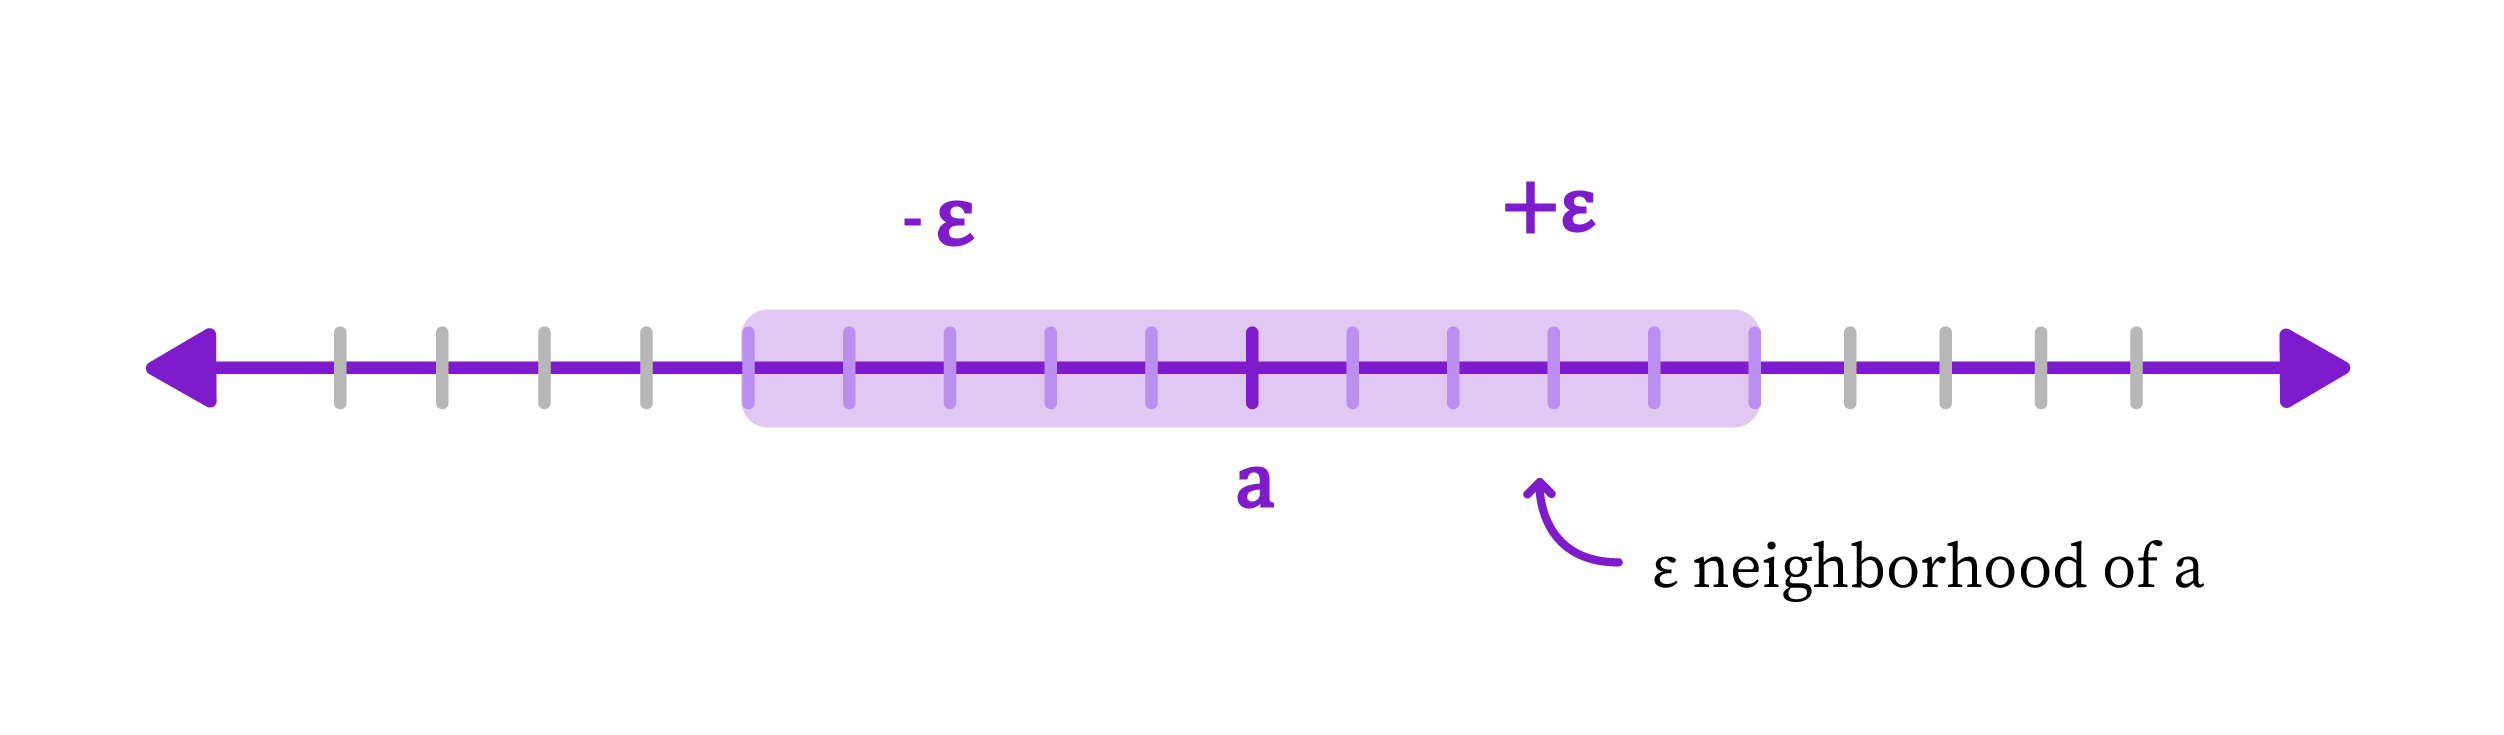
\includegraphics [width=10cm,height=10cm,keepaspectratio]{tex graphs-10.png}
    \caption{$\epsilon$ - Neighborhood}
\end{figure}
\begin{theorem}{}{}
    If $x^*$ belongs to $\epsilon$- neighborhood the $x^* = a $
    \begin{proof}
        $\forall \epsilon > 0, x^*$ belongs to $\epsilon$- neighborhood implies:\\
        $|x^* -a|< \epsilon$ Also $|x^* -a|\geq 0$\\
        Thus, $0<|x^* -a|< \epsilon$\\
        Using theorem \ref{neigh1} :\\
        $|x^* -a|=0 \Rw x^*=a$
    \end{proof}
\end{theorem}
\begin{theorem}{}{}
    Have to prove, $(-1)(-1)=1$
    \begin{proof}
        \begin{align*}
            \text{Here,} &\;1+(-1)=0\\
        \Rw &\;(-1)\{ 1+(-1)\}=0\\
        \Rw &\;(-1)(1)+(-1)(-1)=0 \hs{2cm} \textit{[Distributive property]}\\
        \Rw &\;-1 + (-1)(-1)=0\\
        \Rw &\;-1 + (-1)(-1)+1=0+1\\
        \Rw &\;-1+1+(-1)(-1)=1\\
        \Rw &\;0 +(-1)(-1)=1\\
        \Rw &\;(-1)(-1)=1
        \end{align*}
    \end{proof}
\end{theorem}
$|a|=
\begin{cases}
    a   & \text{if }a\geq 0\\
    -a&\text{if }a<0
\end{cases}
$
\section{Sequences}
A sequence in $\mathbb{R}$ is a function of $\mathbb{N}$ \\
$f:\mathbb{N}\to\mathbb{R}$\\
Symbols of sequence: $x_n,\; (x_n),\;\{x_n\},\; (\;x_n\mathop{)}\limits_{n=1}^\infty$
\subsection*{Convergent sequence}
\begin{theorem}{Convergent sequence}{}
    If $\forall\epsilon>0,\; \exists k \in \mathbb{N}$\; such that $\forall n\geq k\;|x_n-x|<\epsilon$ then $x_n$ converges to x. i.e. $\lim_{n\to\infty}x_n=x$\\\\
\end{theorem}
\begin{figure}[H]
    \centering
    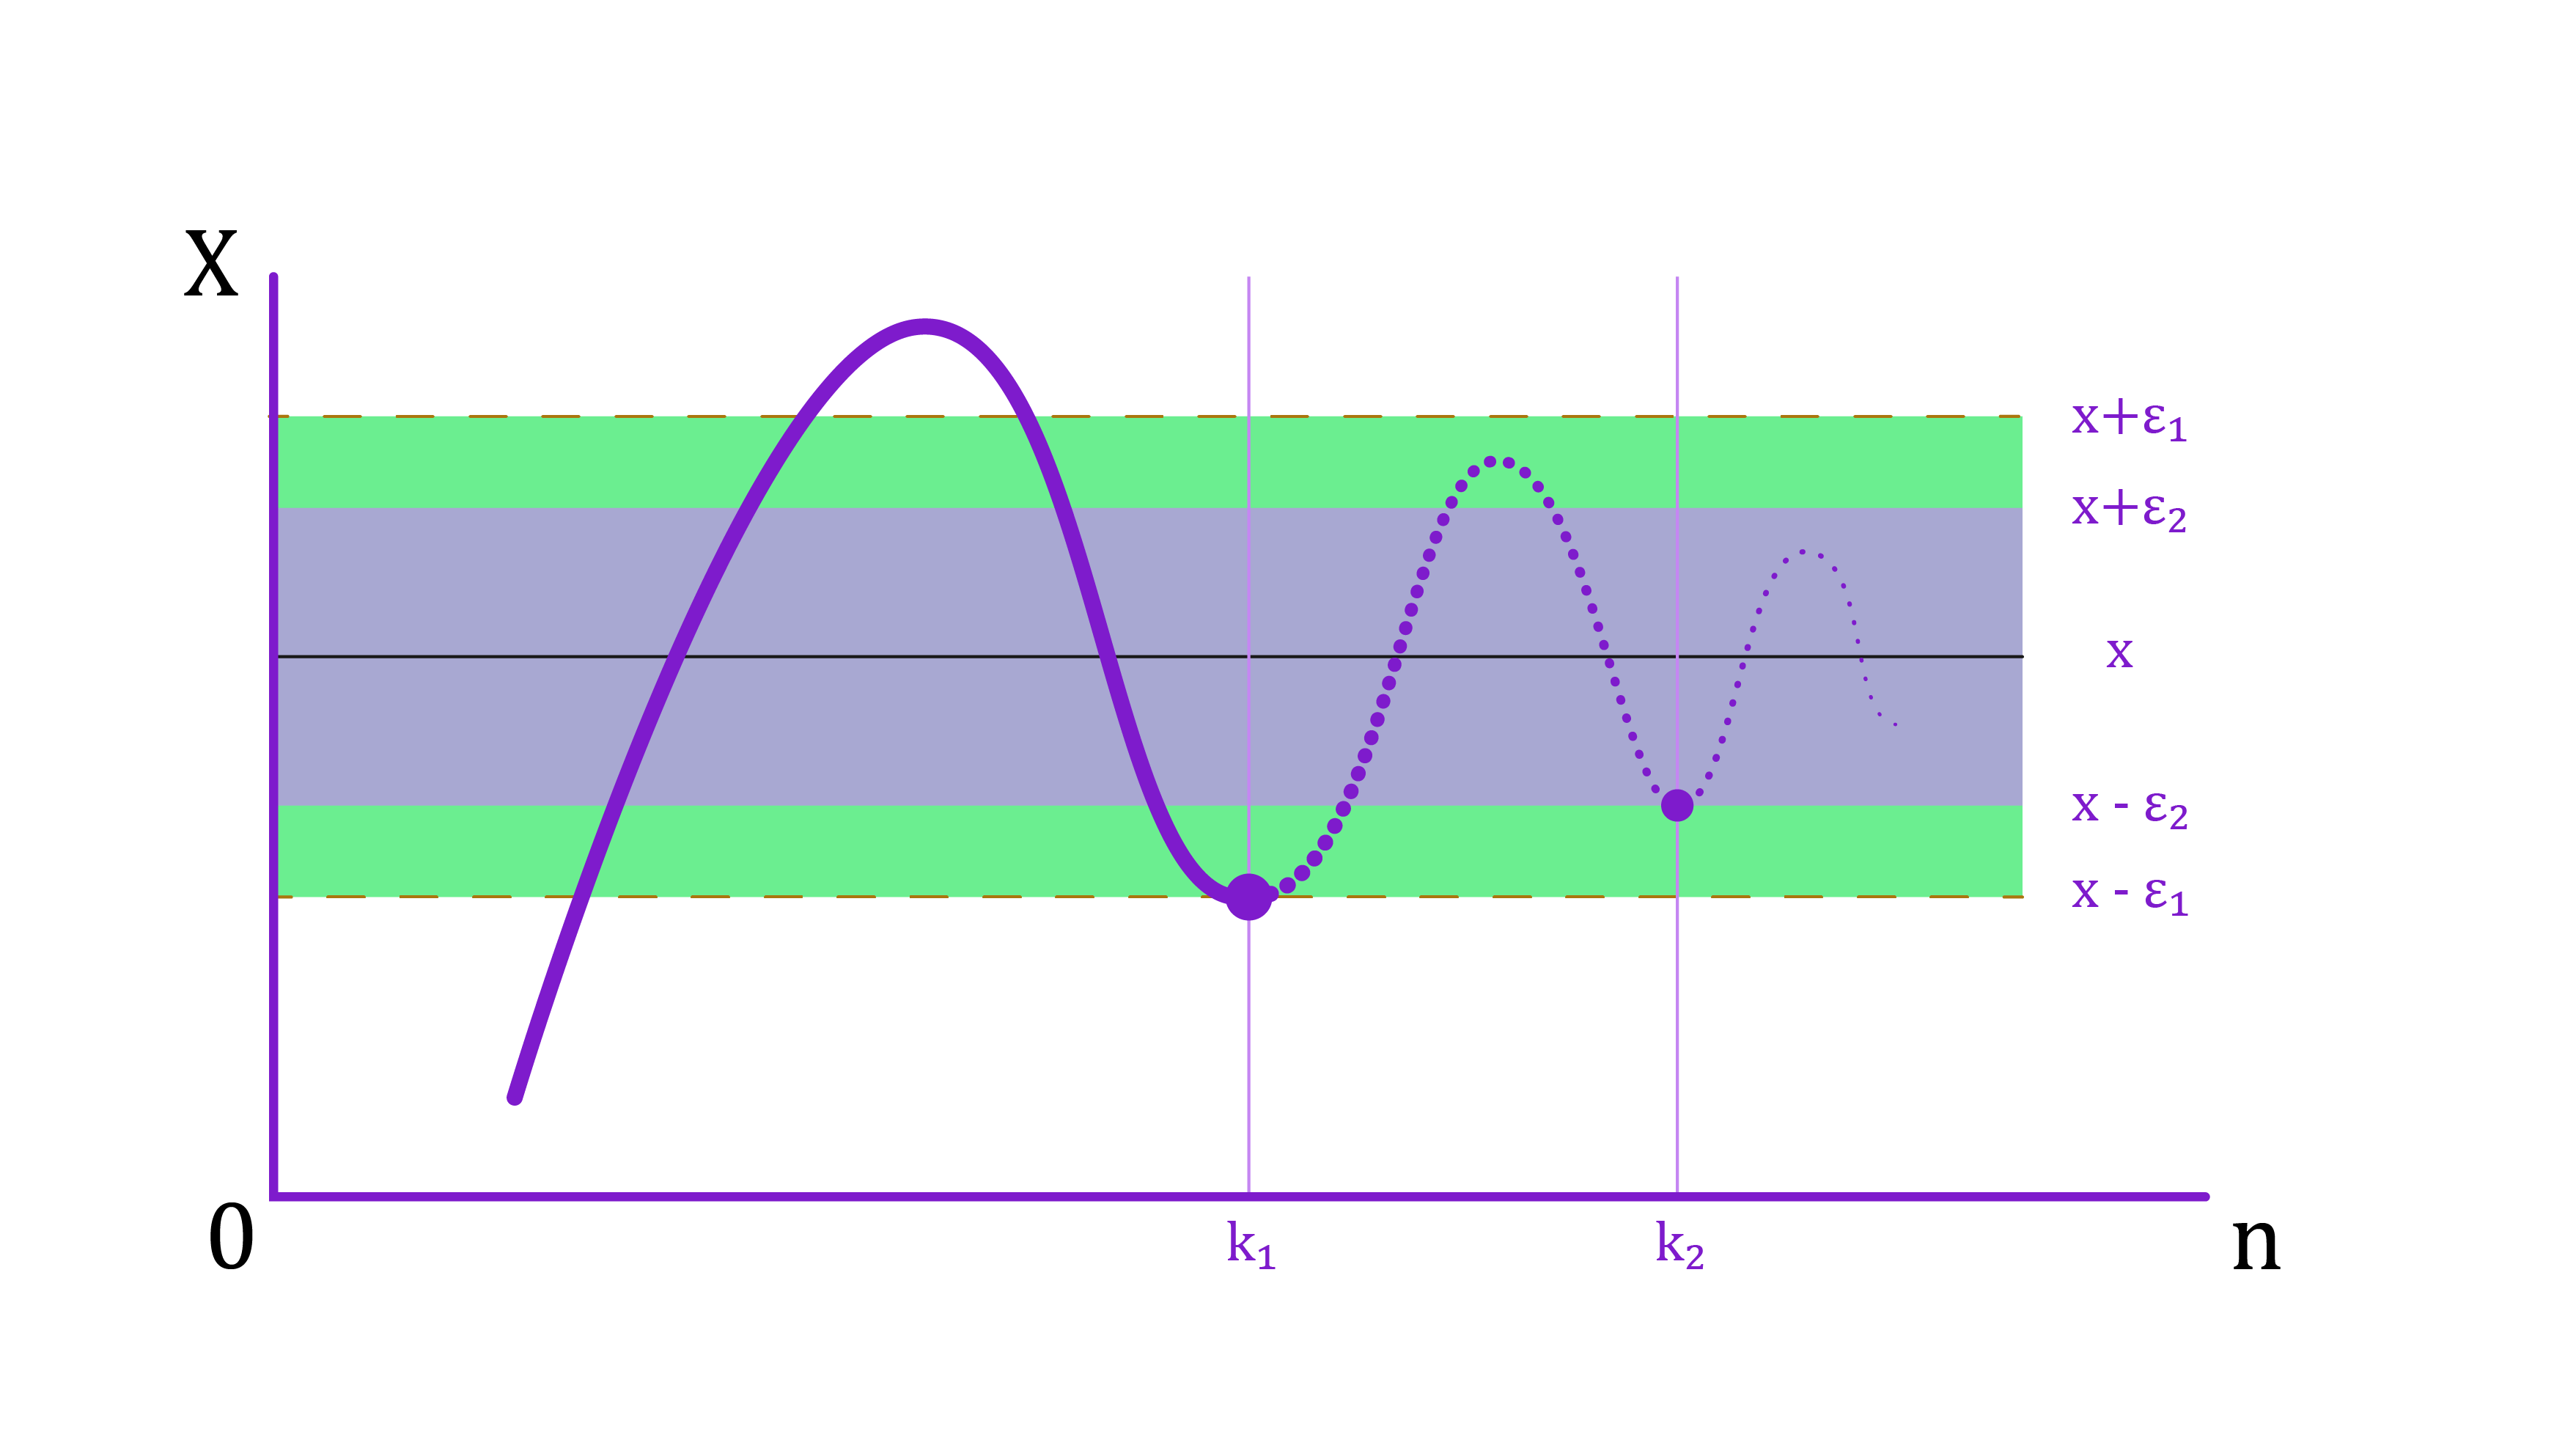
\includegraphics [width=15cm,height=15cm,keepaspectratio]{tex graphs-09.png}
    \caption{Convergence of sequence}
\end{figure}
\begin{example}
    $\lim_{n\to\infty}\frac{1}{1+n^2}=0$\\
    \textit{Solution:} Some Preliminary works - \\
    \begin{align*}
        \text{We want,}\quad & |\frac{1}{1+n^2}|<\epsilon \hs{10cm} \\
        \Rw  \;              & \frac{1}{1+n^2}<\epsilon             \\
        \Rw  \;              & 1+n^2 > \frac{1}{\epsilon}           \\
        \Rw  \;              & n^2 > \frac{1}{\epsilon}-1           \\
        \Rw  \;              & n> \sqrt{\frac{1}{\epsilon}-1}       \\
    \end{align*}
    \textbf{\large Main solution:}\\
    Take any $\epsilon>0$\\
    Choose $k>\sqrt{\frac{1}{\epsilon}-1}$\\
    Now, $\forall n \geq k$\\
    \begin{align*}
        |\frac{1}{1+n^2}-0| & =\frac{1}{1+n^2}\hs{7cm}                                 \\
                            & \leq \frac{1}{1+k^2}                                     \\
                            & < \frac{1}{1+\left(\sqrt{\frac{1}{\epsilon}-1}\right)^2} \\
                            & =\epsilon                          \hs{12cm}\square      \\
    \end{align*}
\end{example}
\begin{example}
    $\lim_{n\to\infty}b^n=0$ \qquad where, $0<b<1$\\
    \textit{Solution:} Some Preliminary works - \\
    \begin{align*}
        \text{We want,}\quad & |x_n-x|,\epsilon    \hs{10cm}            \\
        \Rw\;                & |b^n|<\epsilon                           \\
        \Rw\;                & b^n<\epsilon\qquad[\;\because b^n>0]     \\
        \Rw\;                & n \ln b < \ln\epsilon                    \\
        \Rw\;                & n<\frac{\ln\epsilon}{\ln b}\qquad[error] \\
    \end{align*}
    But n is greater then $\displaystyle\frac{\ln\epsilon}{\ln b}$ as $\ln b <0$\\
    $\displaystyle\therefore n>\frac{\ln\epsilon}{\ln b} $\\\\
    \textbf{\large Main solution:}\\
    Take any $\epsilon>0$\\
    Choose $\displaystyle k>\frac{\ln \epsilon}{\ln b}$\\
    Now, $\forall n \geq k$
    \begin{align*}
        |b^n-0|=|b^n|=b^n\leq b^k
        <b^{\displaystyle (\frac{\ln \epsilon}{\ln b})}
        =e^{\displaystyle \ln b (\frac{\ln \epsilon}{\ln b})}=\epsilon  \hs{7cm}\square
    \end{align*}
\end{example}
\begin{theorem}{}{}
    Convergent sequence has a unique Limit
    \begin{proof}
        Let sequence $x_n$ converges to x and y.\\
        Take any $\epsilon>0$\\
        By definition of convergence,\\
        $\exists K_1 \in \mathbb{N}$\; such that $\forall n \geq k, |x_n-x|<\frac{\epsilon}{2}$\\
        $\exists K_2 \in \mathbb{N}$\; such that $\forall n \geq k, |x_n-y|<\frac{\epsilon}{2}$\\\\
        Choose $K=\max(K_1,K_2)$\\Now, $\forall n\geq k$\\
        \begin{align*}
            |x-y| & =|x-x_n+x_n-y|  \hs{5cm}                        \\
                  & = |(x-x_n)+(x_n-y)|                             \\
                  & \leq |(x-x_n)+(x_n-y)|                          \\
                  & = |x_n-x|+|x_n-y|                               \\
                  & < \frac{\epsilon}{2}+\frac{\epsilon}{2}         \\
                  & = \epsilon                                      \\
            \text{Here}\forall \epsilon>0,\quad 0\leq|x-y|<\epsilon \\
            \text{So,}|x-y|=0 \text{  implies  }x=y
        \end{align*}
    \end{proof}
\end{theorem}
\begin{align*}
    a_n & =\frac{1}{n} & \longleftarrow  \text{ Convergent sequence}\hs*{\fill} \\
    b_n & =n           & \longleftarrow  \text{Divergent sequence}\hs*{\fill}   \\
    x_n & =(-1)^n      & \longleftarrow   \text{Not convergent or divergent}    \\
\end{align*}
\begin{definition}[Bounded Sequence]
    A sequence $x_n$ is bounded if $\forall n \in \mathbb{N},\exists M \in \mathbb{R} $ such that $|x_n|\leq M$\\
\end{definition}
\begin{theorem}{}{}
    Convergent sequence is always bounded
\begin{proof}
    Hw
\end{proof}
\end{theorem}
\subsection*{Limit Theorem}
If $x_n$ and $y_n$ are two sequences such that $\lim_{n\to\infty}x_n=x$ and $\lim_{n\to\infty}y_n=y$ then
\begin{enumerate}
    \item $\displaystyle\lim_{n\to\infty}(x_n+y_n)=x+y$
    \item $\displaystyle\lim_{n\to\infty}(x_n-y_n)=x-y$
    \item $\displaystyle\lim_{n\to\infty}(x_n.y_n)=x.y$
    \item $\displaystyle\lim_{n\to\infty}\frac{x_n}{y_n}=\frac{x}{y}$
\end{enumerate}
\begin{theorem}{Limit theorem}\;
    $\displaystyle\lim_{n\to\infty}(x_n+y_n)=x+y$
\begin{proof}
    $\forall\epsilon>0,\; \exists k \in \mathbb{N}$\; such that $n\geq k\;|x_n+y_n-(x+y)|<\epsilon$\\\\
    Take any $\epsilon >0$\\ By the definition of convergence\\
    $\exists K_1 \in \mathbb{N}$\; such that $\forall n \geq k, |x_n-x|<\frac{\epsilon}{2}$\\
    $\exists K_2 \in \mathbb{N}$\; such that $\forall n \geq k, |x_n-y|<\frac{\epsilon}{2}$\\
    Choose $K=\max(K_1,K_2)$\\Now, $\forall n\geq k$\\
    \begin{align*}
        |x_n+y_n-(x+y)|
         & =|(x_n-x)+(y_n-y)| \hs{4cm}                                                           \\
         & <|x_n-x|+|y_n-y|                       \hs{4cm} \text{[Triangle Inequality $|x+y|<|x|+|y|$]} \\
         & <\frac{\epsilon}{2}+\frac{\epsilon}{2}                                                \\
         & =\epsilon                                                                             \\
    \end{align*}
\end{proof}
\end{theorem}
\begin{theorem}{}{}
    We can write $\displaystyle\lim_{n\to\infty}(x_n-y_n)=x-y$
\end{theorem}
\begin{theorem}{}{}
    we can write $\displaystyle\lim_{n\to\infty}(x_ny_n)=xy$
\begin{proof}
    Take any $\epsilon >0$\\ By the definition of convergence\\
    $\exists K_1 \in \mathbb{N}$\; such that $\forall n \geq k, |x_n-x|<\frac{\epsilon}{2M}$\\
    $\exists K_2 \in \mathbb{N}$\; such that $\forall n \geq k, |x_n-y|<\frac{\epsilon}{2|x|}$\\\\
    Choose $K=\max(K_1,K_2)$\\Now, $\forall n\geq k$\\
    \begin{align*}
        |x_ny_n-(xy)|
         & =|x_ny_n-y_nx+y_nx-xy| \hs{4cm}                                                                 \\
         & =|y_n(x_n-x)+x(y_n-y)|                                                                          \\
         & \leq |y_n||x_n-x|+|x||y_n-y|                    & \text{[Triangle Inequality $|xy|\leq|x||y|$]} \\
         & \leq M |x_n-x|+|x||y_n-y|                       & \text{[$|y_n|\leq M$]}                        \\
         & < M\frac{\epsilon}{2M}+|x|\frac{\epsilon}{2|x|}                                                 \\
         & =\epsilon                                                                                       \\
    \end{align*}
\end{proof}
\end{theorem}
\begin{theorem}{}{}
        We can write $\ds\lim_{n\to\infty}\frac{x_n}{y_n}=\frac{x}{y}$
\begin{proof}
    Preliminary works: \\
    \begin{align*}
        \forall\epsilon>0,\; \exists k \in \mathbb{N}\; \text{such that} \forall n\geq k\; ,|\frac{1}{y_n}-\frac{1}{y}| & <\epsilon \\
        |\frac{y_n-y}{y_n y}|                                                                                           & <\epsilon \\
        \frac{|y_n-y|}{|y_n||y|}                                                                                        & <\epsilon
    \end{align*}
    Now we have to replace the sequence $y_n$ with some constant value.\\
    let, $\alpha = \frac{|y|}{2}>0$\\
    \begin{align*}
        \exists k, \text{such that} \forall n \geq K_1 , & |y_n-y|  <\frac{|y|}{2}                                                                                    \\
        \Rw                                              & -|y_n-y|                                              >-\frac{|y|}{2}                                    \\
        \Rw                                              & -\frac{|y|}{2}                                        < -|y_n-y|                                             \\
        \Rw                                              & -\frac{|y|}{2}                             <-|y_n-n|\leq |y_n|-|y| \hs{1cm}\text{[See corollary \ref{TE}]} \\
        \Rw                                              & \frac{|y|}{2}<|y_n|-|y|                                                                                     \\
        \Rw                                              & \frac{|y|}{2}<|y_n| \hs{2cm}\text{[adding $|y|$ in both sides]}                                             \\
        \Rw                                              & \frac{2}{|y|}>\frac{1}{|y_n|}                                                                             \\
    \end{align*}
    Take any $\epsilon >0$\\\\ By the definition of convergence\\
    $\exists K_2 \in \mathbb{N}$\; such that $\forall n \geq k, |y_n-y|<\ds\frac{\epsilon |y|^2}{2}$\\\\
    Choose $K=\max(K_1,K_2)$\\Now, $\forall n\geq k$\\
    \begin{align*}
        |\frac{1}{y_n}-\frac{1}{y}| & =\frac{|y_n-y|}{|y_n||y|}     \hs{6cm} \\
                                    & <\frac{2|y_n-y|}{|y||y|}               \\
                                    & <2 \frac{\epsilon |y|^2}{2|y|^2}       \\
                                    & =\epsilon
    \end{align*}
\end{proof}
\end{theorem}
\begin{corollary}\label{TE}
    Corollary of Triangle Inequality\\
    \begin{align*}
        ||a|-|b||  & \leq |a-b|\\
        \Rw -|a-b| & \leq |a|-|b|\leq |a-b| \hs{3cm}  \text{[$|a|\leq b \Rw -b\leq a \leq b$]} \\
    \end{align*}
\end{corollary}
\begin{theorem}{Sandwich or Squeeze theorem}\\
    let $x_n,\; y_n$ and $z_n$ are three sequences such that $x_n<y_n<z_n$\\
    if $\lim_{n\to\infty}x_n=w$ and $\lim_{n\to\infty}z_n=w$ then $\lim_{n\to\infty}y_n=w$
\begin{proof}
    Take any $\epsilon >0$\\
    $\exists K_1 \in \mathbb{N}$\; such that $\forall n \geq k_1, |x_n-w|<\epsilon$\\
    $\exists K_2 \in \mathbb{N}$\; such that $\forall n \geq k_2, |z_n-w|<\epsilon$\\
    We can write
    \begin{align}
        \label{ep1} -\epsilon<x_n-w<\epsilon \\
        \label{ep2} -\epsilon<z_n-w<\epsilon
    \end{align}
    Choose $K=\max(k_1,k_2)$\\
    \begin{gather*}
        \text{Here,\;}\forall n \geq K    \hs{10cm} \\
        x_n\leq y_n \leq z_n                 \\
        x_n-w\leq y_n -w\leq z_n-w                   \\
        \hs{2.5cm}-\epsilon<x_n-w\leq y_n -w\leq z_n-w<\epsilon \qquad \text{[from (\ref{ep1}) and (\ref{ep2}) ]}  \\
        -\epsilon< y_n-w<\epsilon  \\
        |y_n -w|<\epsilon
    \end{gather*}
\end{proof}
\end{theorem}
\begin{example}
    $x_n=\displaystyle\frac{\sin{n}}{n}$
    \begin{gather*}
        -1\leq \sin{n} \leq 1 \\
        -\frac{1}{n}\leq \frac{\sin n}{n}\leq \frac{1}{n}\\
        \lim_{n\to\infty}-\frac{1}{n}\leq \lim_{n\to\infty}\frac{\sin n}{n}\leq\lim_{n\to\infty} \frac{1}{n}\\
        0\leq \lim_{n\to\infty}\frac{\sin n}{n}\leq 0\\
    \end{gather*}
    By squeeze theorem: $\displaystyle\lim_{n\to\infty}\frac{\sin n}{n}=0$
\end{example}
\begin{figure}
    \centering
    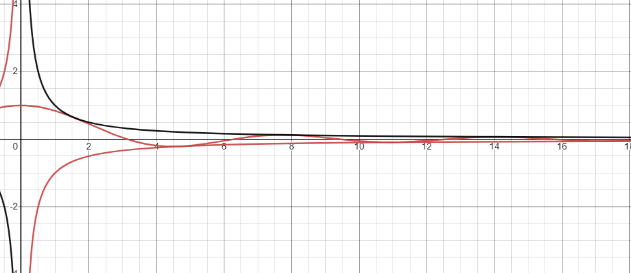
\includegraphics{sin(n)n.png}
    \caption{Graph of $\frac{\sin n}{n} (Sinc function)$}
    \label{fig:mylabel}
\end{figure}
\begin{example}
    $\displaystyle\lim_{(x,y)\to(0,0)}\frac{x^2y}{x^2+y^2}$
    \begin{gather}
        0\leq \frac{x^2}{x^2+y^2} \leq 1 \label{sq1}\\
        -|y|\leq y\leq |y| \label{sq2}
    \end{gather}
    Multiplying equation (\ref{sq1}) and (\ref{sq2})\\
    \begin{gather*}
        -|y|\leq \frac{x^2y}{x^2+y^2}\leq |y|\\
        \displaystyle\lim_{(x,y)\to(0,0)}-|y|\leq \displaystyle\lim_{(x,y)\to(0,0)}\frac{x^2y}{x^2+y^2}\leq \displaystyle\lim_{(x,y)\to(0,0)}|y|\\
        \hspace{4cm}0\leq\displaystyle\lim_{(x,y)\to(0,0)}\frac{x^2y}{x^2+y^2}\leq 0  \hspace{5cm} \square
    \end{gather*}
\end{example}\vs{0.75cm}
\textbf{Question:} If two sequences are convergent then what would their addition sequence be?\\
\textbf{Question:} If one sequence is convergent and another is divergent what would that be?
\subsection{Sub-sequence:}
Sub-sequence is a part of any sequence.\\
Let $x_n$ be a sequence and $n_1,n_2,n_3,....,n_k$ is increasing natural number.\\\\
Sequence of $x_n$ will be $(X_{n_k}): X_{n_1},X_{n_2},X_{n_3},...,X_{n_k}$\\
\begin{align*}
    \textbf{Sequence: }     & \displaystyle\frac{1}{n}: 1,\frac{1}{2},\frac{1}{3},\frac{1}{3},\frac{1}{4},...\hspace{8cm}    \\
    \textbf{Sub-Sequence: } & \displaystyle\frac{1}{n}: 1,\frac{1}{4},\frac{1}{10},\frac{1}{12},\frac{1}{15},...\hspace{8cm}
\end{align*}
Elements of sub sequence maintain order. And the starting element should not necessarily be the same element as that of the sequence. If the sequence in infinite then the sub-sequence should also be infinite. If the sequence is convergent then sub sequence should also be convergent.\\\\
Difference between a subset and sub-sequence is that it is not necessary to maintain order in subset. But it is not the case for sub-sequence.
\begin{align*}
    \textbf{Sequence: }     & 1,-1,1,-1,1,-1,1,-1,...\hspace{8cm}             \\
    \textbf{Sub-Sequence: } & 1\;,1\;,1\;,1\;,1\;,1\;,1\;,1\;,...\hspace{8cm} \\
    \textbf{Sub-Sequence: } & -1,-1,-1,-1,-1,-1,...\hspace{8cm}               \\
    \textbf{Sub-Sequence: } & 1,-1,-1,-1,1,...\hspace{8cm}                    \\
\end{align*}
If sequence is not convergent then we can not guarantee that sub-sequences are not convergent. We can not dictate its nature.
\begin{theorem}{Bolzano-weierstrass Theorem}{} Bounded sequence will have a convergent sub-sequence.\\
\end{theorem}
\begin{definition}[Cauchy sequence]
    A sequence $(x_n)$ is cauchy sequence if $\forall \epsilon > 0, \exists k \in \mathbb{N},$ such that $\forall n,m \geq k,\ |x_n -x_m|< \epsilon$
\end{definition}
\begin{example}
    $\frac{1}{n}$ is cauchy sequence\\
    solution.\ Take any $\epsilon > 0$\\
    Choose $\displaystyle k>\frac{2}{\epsilon}$\\
    Then, $\forall n,m \geq k$
    \begin{align*}
        |\frac{1}{n}-\frac{1}{m}|&\leq |\frac{1}{n}|+|\frac{1}{m}|\hs{9cm}\\
        &= \frac{1}{n}+\frac{1}{m}\\
        &\leq \frac{1}{k}+\frac{1}{k}\\
        &= \frac{2}{k}\\
        &<{\epsilon}\hspace{5cm} \square
    \end{align*}
\end{example}
\begin{theorem}{}{}
    If a sequence is convergent, then it is cauchy sequence.\\
    \textit{[For cauchy sequence we have to show $\forall \epsilon > 0, \exists k \in \mathbb{N},$ such that $\forall n,m \geq k,\ |x_n -x_m|< \epsilon$]}\begin{proof}
        Take any $\epsilon >0$\\
        By the definition of convergence, $\exists k_1 \in \mathbb{N}$ such that $\forall n \geq k,\ |x_n -x|< \displaystyle \frac{\epsilon}{2}$\\
        Choose $k\geq k_1$\\
        Now, $\forall n,m \geq k $
        \begin{align*}
            |x_n -x|&= |(x_n -x)-(x_m -x)|\\
            &\leq |x_n -x|-|x_m -x| \hs{4cm}\text{[Triangular inequality of absolute value]}\\
            &< \frac{\epsilon}{2}+ \frac{\epsilon}{2}\\
            &= \epsilon
        \end{align*}
    \end{proof}
\end{theorem}
\begin{theorem}{}{}
    Every cauchy sequence is bounded.
    \begin{proof}
        Home work
    \end{proof}
\end{theorem}
\begin{theorem}{}{}
    Every cauchy sequence is convergent.
    \begin{proof}
        Let $(x_n)$ be any cauchy sequence.\\
        We know that cauchy sequences are bounded. so by "Bolzano-weierstrass Theorem" cauchy sequence must have a convergent subsequence.\\\\
        Take any $\epsilon >0$\\
        By the definition of convergence, $\exists k_1 \in \mathbb{N}$ such that $\forall n,m \geq k,\ |x_n -x|< \ds \frac{\epsilon}{2}$\\\\
        Let $\ds x_{n_k}$be the subsequence that is convergent to x.\\
        By the definition of convergence,$\exists k_2 \in \mathbb{N}$ such that $\forall n_k \geq k_2,\ |x_{n_k} -x|< \ds \frac{\epsilon}{2}$\\\\
        Choose $k=\max[k_1,k_2]$\\
        Now, $\forall n \geq k,$
        \begin{align*}
            |x_n-x|&=|(x_n-x_{n_k})+(x_{n_k}-x)| \hs{7cm}\\
            &\leq |x_n-x_{n_k}|+|x_{n_k}-x|\\
            &= |x_n-x_m|+|x_{n_k}-x|\\
            &< \frac{\epsilon}{2}+\frac{\epsilon}{2}\\
            &= \epsilon\\
        \end{align*}   
    \end{proof}
\end{theorem}
\vs{1cm}
\section{Series}
Sum of a set of numbers or terms are called series.\\
\textbf{Notation:} $\ds \sum_{i=1}^{\infty} x_i = S_n\ \longleftarrow $ sum of n terms\\\\
\tabto{4cm} \textbf{Series:}\hs{2cm}
\begin{align*}
    S_1&=x_1\\
    S_2&=x_1 +x_2\\
    S_3&=x_1+x_2+x_3\\
    ...\\
    S_n&=x_1+x_2+x_3+...+x_n\\
\end{align*}
\tabto{4cm}\textbf{Sequence:} $(x_n)$\\
\begin{align*}
    S_1,S_2,S_3,......,S_n
\end{align*}
\begin{example}
    If $\ds (x_n)_{n=1}^\infty=x^n$ show that $|x|<1$ Then the geometric series $\ds \sum_{n=0}^{\infty} x^n$ converges to $\frac{1}{1-x}$\\
    \textit{Solution:}\\
    \begin{align}
        S_n=\sum_{n=0}^{\infty} x^n= 1+x+x^2+x^3+...+x^n \label{sn}\\
        x.S_n=\sum_{n=0}^{\infty} x^n= x+x^2+x^3+...+x^n+x^{n+1} \label{xsn}
    \end{align}
    Subtracting (\ref{xsn}) from (\ref{sn})\\
    \begin{align*}
        &S_n-xS_n=1 \hs{7cm}\\
        \Rw \;& S_n(1-x)=1-x^{n+1}\\
        \Rw \;& S_n= \ds \frac{1-x^{n+1}}{1-x}
    \end{align*}
    Taking the limit,
    \begin{align*}
        \lim_{n\to\infty} S_n &=\lim_{n\to\infty} \ds \frac{1-x^{n+1}}{1-x}\hs{7cm}\\
        &= \ds \frac{\ds \lim_{n\to\infty} (1-x^{n+1})}{\ds\lim_{n\to\infty} (1-x)}\hs{3cm}\text{[Both (1-x) and its limit can not be zero]}\\
        &= \frac{\ds\lim_{n\to\infty}(1)-\ds\lim_{n\to\infty}(x^{n+1})}{\ds\lim_{n\to\infty}(1)-\ds\lim_{n\to\infty}(x)}\\
        &=\frac{1-0}{1-x}\hs{3cm}\text{[$\lim b^n=0;\quad when \ |b|<1$]}\\
        &=\frac{1}{1-x}\hspace{5cm} \square
    \end{align*}
\end{example}\vs{0.5cm}
\begin{example}
    Find the limit of $\ds\sum_{n=1}^{\infty}\frac{1}{n(n+1)}$\\
    \textit{Solution:}\\
    \begin{align*}
        \frac{1}{k(k+1)}+\frac{1}{k+1}=\frac{1}{k}\\
        \frac{1}{k(k+1)}=\frac{1}{k}-\frac{1}{k+1}
    \end{align*}
    Now, The value of $\ds \frac{1}{k(k+1)}$ \\
    \begin{align*}
        \text{When, } k&=1\qquad \frac{1}{k}-\frac{1}{k+1}=\frac{1}{1}-\frac{1}{2}\\
        k&=2\qquad \frac{1}{k}-\frac{1}{k+1}=\frac{1}{2}-\frac{1}{3}\\
        k&=3\qquad \frac{1}{k}-\frac{1}{k+1}=\frac{1}{3}-\frac{1}{4}\\
        & ...\qquad ...\\
        k&=n\qquad \frac{1}{k}-\frac{1}{k+1}=\frac{1}{n}-\frac{1}{n+1}
    \end{align*}
    \begin{align*}
        \sum_{n=1}^{n} \frac{1}{k(k+1)}=1-\frac{1}{n+1}\\\\
        \lim_{n\to\infty} S_n &= \lim_{n\to\infty}(1-\frac{1}{n+1})\\
        &= \lim_{n\to\infty}(1)-\lim_{n\to\infty}(\frac{1}{n+1})\\
        &= 1-\frac{\lim_{n\to\infty}(1)}{\lim_{n\to\infty}(n+1)}\\
        &= 1-\frac{1}{\infty}\\
        &= 1
    \end{align*}
    \subsection{Comparison Test}
    Let $x_n$ and $y_n$ be two sequences such that, $0\leq x_n\leq y_n,\ \forall n \geq k$ \begin{itemize}
        \item Then convergence of $\sum y_n$ implies convergence of $\sum x_n$
        \item Divergence of $\sum x_n$ implies divergence of $\sum y_n$
    \end{itemize}
\textbf{HW examples of comparison test $\sum_{n=1}^{}\infty$ converges}\\
\begin{example}
    Show $\ds \sum_{n=1}^{\infty}\frac{1}{n}$ diverges.
    \textit{Solution: }
    \begin{align*}
        {\ds \sum_{n=1}^{\infty}\frac{1}{n}}&=1+\frac{1}{2}+\frac{1}{3}+\frac{1}{4}+\frac{1}{5}+\frac{1}{6}+\frac{1}{7}+\frac{1}{8}+\frac{1}{9}+\frac{1}{10}+\frac{1}{11}+...\\
        &>\frac{1}{2^0}+\frac{1}{2^1}+\frac{1}{2^2}+\frac{1}{2^2}+\frac{1}{2^3}+\frac{1}{2^3}+\frac{1}{2^3}+\frac{1}{2^3}+\frac{1}{2^4}+\frac{1}{2^4}+\frac{1}{2^4}+...\\
        & \hs{2cm}\text{[Replacing each denominator with the next largest power of 2]}\\
        &=1+\frac{1}{2}+\frac{1}{2}+\frac{1}{2}+\frac{1}{2}+\frac{1}{2}+\frac{1}{2}+\frac{1}{2}+... \ ...+\infty
    \end{align*}
    Since, $\ds 1+\frac{1}{2}+\frac{1}{2}+\frac{1}{2}+\frac{1}{2}+...$ diverges, using comparison text $\ds \sum_{n=1}^{\infty}\frac{1}{n}$ will also diverge.
\end{example}
\end{example}
\vs{.5cm}
\section{Metric Space}
A metric space $(S,D)$ is a set \textbf{S} together with a distance function \textbf{d} such that
\begin{enumerate}
    \item $d(x,y)\geq 0, \forall x,y \in S$
    \item $d(x,y)=0, \Leftrightarrow x=y, \forall x,y \in S$
    \item $d(x,y) = d(y,x)$
    \item $d(x,y)\leq d(x,z)+d(z,y),\ \forall x,y,z \in S$
\end{enumerate}
\vs{0.75cm}
\begin{example}
    $(\mathbb{R},d)$ is a metric space with $d=|x-y| \ \forall x,y \in \mathbb{R}$\\
    \textit{Solution:} 
    \begin{enumerate}
        \item $d=|x-y| \geq 0 \hs{1cm}\text{[By definition of absolute value]}$
        \item $|x-y|=0 \Rw x-y=0 \Rw x=y$\\
        Again, $x=y \Rw x-y=0 \Rw |x-y|=0$
        \item $|x-y|=|y-x|$
        \item $|x-y|=|(x-y)-(y-z)|\leq |x-z|+|y-z|$ \qquad [By triangular inequality of absolute value]
    \end{enumerate}
\end{example}
\vs{0.75cm}
\begin{example}
    $(\mathbb{R}^2,d)$ is a metric space with $\ds d(p_1,p_2)=\sqrt{(x_1-x_2)^2+(y_1-y_2)^2}$
    \begin{enumerate}
        \item hw
        \item hw
        \item hw
        \item 
        \begin{align*}\ds
            d(p_1,p_2)&=\sqrt{(x_1-x_2)^2+(y_1-y_2)^2}\\
            &=\sqrt{\{(x_1-x_3)+(x_3-x_2)\}^2+\{(y_1-y_2)+(y_3-y_2)\}^2}\\
            &\leq \sqrt{(x_1-x_3)^2+(y_1-y_3)^2}+\sqrt{(x_3-x_2)^2+(y_3-y_2)^2}\hs{1cm}\text{[Minkowski inequality]}\\
            &= d(p_1,p_3)+d(p_2,p_3)
        \end{align*}
        \textbf{Minkowski inequality:} $\sqrt{\sum (m_i+n_i)^2}\leq \sqrt{\sum {m_i}^2}+\sqrt{\sum {n_i}^2}$
    \end{enumerate}
\end{example}
\vs{0.75cm}
\begin{example}
    $(\mathbb{R}^2,d)$ is a metric space with $\ds d(p_1,p_2)=|x_1-x_2|+|y_1-y_2|$\\
    \textit{Solution:}\\
    \begin{enumerate}
        \item hw
        \item hw
        \item hw
        \item We have to show $d(p_1,p_2)\leq d(p_1,p_3)+d(p_2,p_3)$
            \begin{align*}
                d(p_1,p_2)&=|x_1-x_2|+|y_1-y_2|\\
                &=|x_1-x_3+x_3-x_2|+|y_1-x_3+x_3-y_2|\\
                &\leq \{|x_1-x_3|+|x_3-x_2|\}+\{|y_1-x_3|+|x_3-y_2|\}\hs{1cm}\text{[Triangular inequality]}\\
                &= d(p_1,p_3)+d(p_2,p_3)
            \end{align*}
    \end{enumerate}
\end{example}
\vs{0.75cm}
\begin{align*}
    & 1+\frac{1}{2^2}+\frac{1}{3^2}+\frac{1}{4^2}+\frac{1}{5^2}+\frac{1}{6^2}+\frac{1}{7^2}+\frac{1}{8^2}+\frac{1}{9^2}+\frac{1}{10^2}+\frac{1}{11^2}+\frac{1}{12^2}+\frac{1}{13^2}+\frac{1}{14^2}+\frac{1}{15^2}+...\\
    &< 1+\textcolor{blue}{\frac{1}{2^2}+\frac{1}{2^2}}+\textcolor{red}{\frac{1}{4^2}+\frac{1}{4^2}+\frac{1}{4^2}+\frac{1}{4^2}}+\textcolor{blue}{\frac{1}{8^2}+\frac{1}{8^2}+\frac{1}{8^2}+\frac{1}{8^2}+\frac{1}{8^2}+\frac{1}{8^2}+\frac{1}{8^2}+\frac{1}{8^2}}+...\\
    &=1+\frac{1}{2}+\frac{1}{4}+\frac{1}{8}+\frac{1}{16}+\frac{1}{32}+...\\
    &=\ds \left(\frac{1}{2}\right)^0+\left(\frac{1}{2}\right)^1+\left(\frac{1}{2}\right)^2+\left(\frac{1}{2}\right)^3+\left(\frac{1}{2}\right)^4+\left(\frac{1}{2}\right)^5+\left(\frac{1}{2}\right)^6+
\end{align*}
Limit of the series is $\ds \frac{1}{1-\ds\frac{1}{2}}=2$ \qquad As we know
[$\ds 1+r+r^2+r^3+r^4+...=\frac{1}{1-r}; \ |r|<1$]\\

\end{document}